\chapter{Polynomial Kernel SVM}
\label{chap:polynomial_svm}

In this chapter, we extend our analysis to non-linear decision boundaries by leveraging the "Kernel Trick". Instead of explicitly expanding the features into a higher-dimensional space (as we did with Quadratic Logistic Regression), we use a Kernel function $k(x_1, x_2)$ to compute the dot products directly in the dual formulation. 

For this experiment, we utilize the Polynomial Kernel defined as:
\begin{equation}
    k(x_1, x_2) = (x_1^T x_2 + c)^d + \xi
\end{equation}
We set the constant $c = 1$ and the bias regularization parameter $K = 0.0$. Because the expansion of $(x_1^T x_2 + 1)^d$ inherently includes all lower-order terms and a constant, the polynomial kernel already provides an implicit bias offset, rendering the explicit $K$ augmentation unnecessary.

\section{Quadratic Polynomial Kernel ($d=2$)}

\subsection*{What do you obtain when applying a Polynomial Kernel of degree 2?}

Evaluating the Quadratic Kernel over the $C$ hyperparameter space yields the performance metrics shown in Figure \ref{fig:poly_svm_d2}.

\begin{figure}[H]
    \centering
    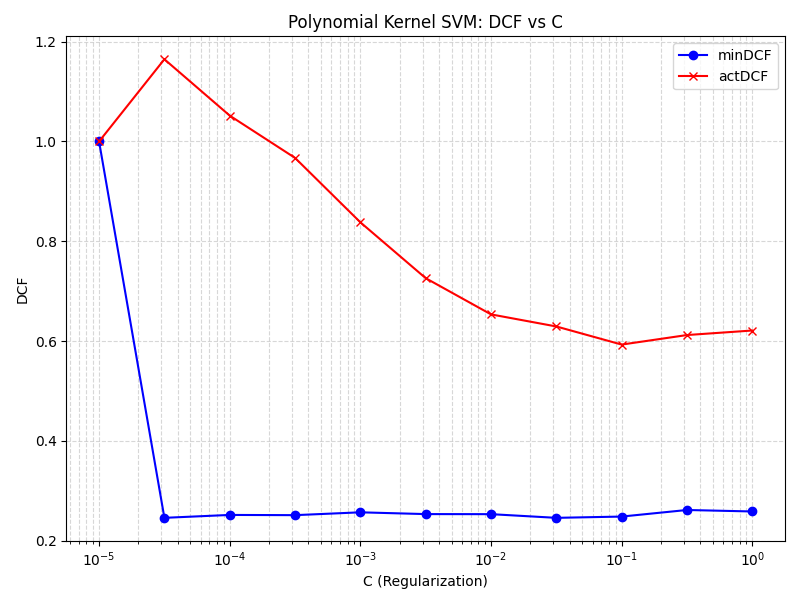
\includegraphics[width=0.85\textwidth]{Poly_Kernel_SVM_DCF_vs_C.png}
    \caption{Actual DCF and Minimum DCF as a function of $C$ for the Polynomial Kernel SVM ($d=2, c=1, K=0, \pi_T = 0.1$).}
    \label{fig:poly_svm_d2}
\end{figure}

The discriminatory power of the quadratic kernel is vastly superior to the linear model. As $C$ varies, the Minimum DCF reaches an optimal value of \textbf{0.2455} at $C=3.16 \times 10^{-2}$. However, the Actual DCF deviates significantly, reaching \textbf{0.6291} at the same operational point, demonstrating a lack of native calibration.

\subsection*{Why does the quadratic boundary perform so well on this dataset?}

The massive improvement in minDCF (dropping from $\approx 0.358$ in the Linear SVM to $0.2455$ here) mathematically proves that the true separation between the "Fake" and "Genuine" classes is inherently non-linear. 

As established in previous laboratories, the classes in this project dataset possess fundamentally different covariance structures (e.g., varying geometric spreads). A linear hyperplane cannot capture differences in variance. By applying a polynomial kernel of degree $d=2$, the SVM natively computes a quadratic decision boundary in the original feature space. This allows the model to separate the classes based on their geometric spread, perfectly mirroring the theoretical advantage of the unconstrained Generative MVG and Quadratic Logistic Regression.

\section{Higher-Degree Polynomial Kernel ($d=4$)}

To test the robustness of the model, we increase the polynomial degree to $d=4$, vastly expanding the capacity of the classifier.

\subsection*{What happens when the polynomial degree is increased to $d=4$?}

The evaluation of the $d=4$ kernel yields the highly volatile trends plotted in Figure \ref{fig:poly_svm_d4}.

\begin{figure}[H]
    \centering
    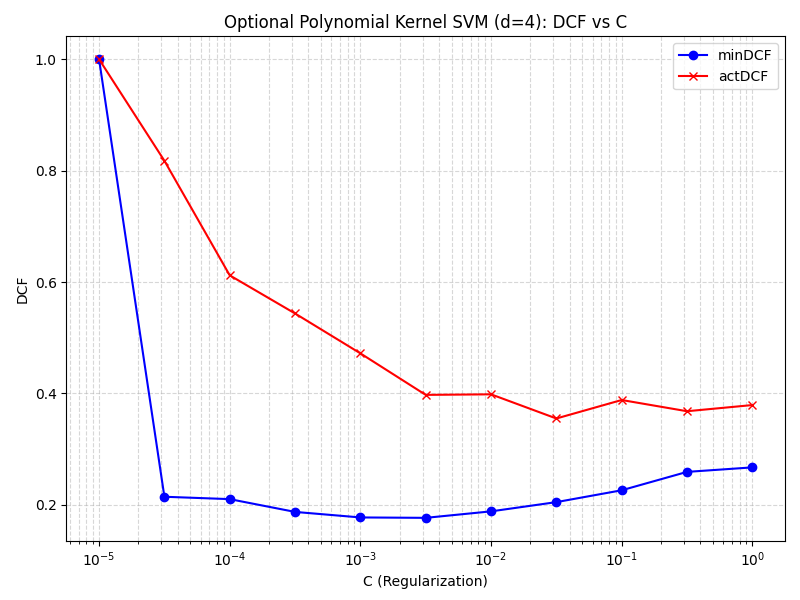
\includegraphics[width=0.85\textwidth]{Poly_Kernel_SVM_d4_DCF_vs_C.png}
    \caption{Actual DCF and Minimum DCF as a function of $C$ for the Polynomial Kernel SVM ($d=4, c=1, K=0, \pi_T = 0.1$).}
    \label{fig:poly_svm_d4}
\end{figure}

For a low value of $C$ ($3.16 \times 10^{-3}$), the model achieves a remarkable Minimum DCF of \textbf{0.1767} and an Actual DCF of \textbf{0.3975}. However, as $C$ increases beyond this point, both metrics degrade catastrophically, indicating a severe loss of both ranking ability and calibration.

\subsection*{How does the interplay between $d$ and $C$ cause this behavior?}

This experiment provides a textbook demonstration of the bias-variance trade-off and catastrophic overfitting:

\begin{itemize}
    \item \textbf{The Risk of High Degree ($d=4$):} Expanding the feature space to the 4th degree grants the SVM massive capacity, allowing it to draw highly complex, wavy boundaries. While this complexity initially discovers a superior geometric fit (minDCF $0.1767$), it makes the model extremely sensitive to the specific noise of the training data.
    \item \textbf{The Role of $C$ in Overfitting:} In Kernel SVMs, a high $C$ heavily penalizes margin violations ($\xi_i$). When combined with the massive flexibility of $d=4$, a high $C$ forces the SVM to contort its high-degree boundary to perfectly wrap around every single training outlier to avoid the penalty. This completely destroys the generalization of the boundary, leading to the massive spike in validation error (DCF) observed in Figure \ref{fig:poly_svm_d4}.
\end{itemize}

Ultimately, $d=2$ provides the optimal structural assumption for this dataset, capturing the necessary covariance interactions without supplying enough mathematical capacity to overfit the noise.